\RequirePackage{flashmovie}
% it is necessary to use "\RequirePackage{flashmovie}" because beamer
% also uses "\pdfminorversion". see flashmovie.sty for an explanation.
\documentclass{beamer}
\usepackage[T1]{fontenc}
\usepackage[utf8]{inputenc}
\usepackage{amsmath,bm}
\usepackage{tikz}
\usetikzlibrary{shapes,arrows}
\tikzstyle{decision} = [diamond, draw, fill=blue!20, 
    text width=4.5em, text badly centered, node distance=2cm, inner sep=0pt]
\tikzstyle{block} = [rectangle, draw, fill=blue!20, 
    text width=5em, text centered, rounded corners, minimum height=4em]
\tikzstyle{line} = [draw, -latex']
\tikzstyle{cloud} = [draw, ellipse,fill=red!20, node distance=3cm, minimum height=2em]
    
\usetheme{Boadilla} % CambridgeUS  %Boadilla
\usepackage{natbib}
%gif :
%\usepackage{movie15}
\usepackage{graphicx}
%\usepackage{epstopdf}
\usepackage{animate}
\usepackage{media9}
\usepackage{float}
\usepackage{braket}
%\epstopdfDeclareGraphicsRule{.gif}{png}{.png}{convert gif:#1 png:\OutputFile}
%\AppendGraphicsExtensions{.gif}
\newcommand{\tbm}[1]{\bm{\tilde{#1}}}
\newcommand{\hbm}[1]{\bm{\hat{#1}}}
\newcommand{\pxth}[2]{p(\bm{#1}_{t};\hbm{#2}_0)}
\newcommand{\pxtt}[3]{p(\bm{#1}_{t};\hbm{#2}_{#3}^i)}

\newcommand{\tc}[1]{\tilde{\mathcal{#1}}}
\newcommand{\mc}[1]{\mathcal{#1}}

\newcommand{\iyx}[2]{\bm{I}(\bm{#1},\bm{#2})}
\newcommand{\iyt}[2]{\bm{I}(\bm{#1},\tbm{#2})}
\newcommand{\pyx}[2]{p(\bm{#1}|\bm{#2})}
\newcommand{\ptx}[2]{p(\tbm{#1}|\bm{#2})}

\newcommand{\argmin}{\arg\!\min}
%\bibliographystyle{agu04}
% make bibliography entries smaller
\renewcommand\bibfont{\scriptsize}
% If you have more than one page of references, you want to tell beamer
% to put the continuation section label from the second slide onwards
%\setbeamertemplate{frametitle continuation}[from second]
% Now get rid of all the colours
%\setbeamercolor*{bibliography entry title}{fg=blue}
%\setbeamercolor*{bibliography entry author}{fg=blue}
%\setbeamercolor*{bibliography entry location}{fg=blue}
%\setbeamercolor*{bibliography entry note}{fg=blue}
% and kill the abominable icon
\setbeamertemplate{bibliography item}{}
\title{\textbf{Dreem project: supervised learning on EEG signals for sleep stage detection }\\}%\texttt{flashmovie} package}
\author{Shuyu Dong , Oussama Ennafii}
% - Give the names in the same order as the appear in the paper.
% - Use the \inst{?} command only if the authors have different
%   affiliation.
\institute[Telecom Paris, MVA] % (optional, but mostly needed)
{
  %\inst{1}%
%  ProjetLibre \\
  MVA project\\
  
  \vspace{1cm}
  %\and
  %\inst{2}%
  
  %\and
  %\inst{3}
  
   }
\date{March 2015}
\begin{document}
\frame{\maketitle}

\section{ Problematic }
\begin{frame}{ Detection of k-complex structures in EEG signals }{}
 %\textbf{Speaker features}:
 \textbf{ Dataset } \\
   \begin{itemize}
   \item { Labeled set: $N = 69,550$ examples of EEG signals and labels(positive and negative) : each example corresponds to 3 seconds' signal sampled at 200Hz.
%   \pause
   }
   \item { Labeled set's positive/negative ratio: $4,861 / 64,689 $. 
   } 
       \end{itemize}
       \begin{figure}[H]
\centering
\makebox[.4\textwidth][c]{         
 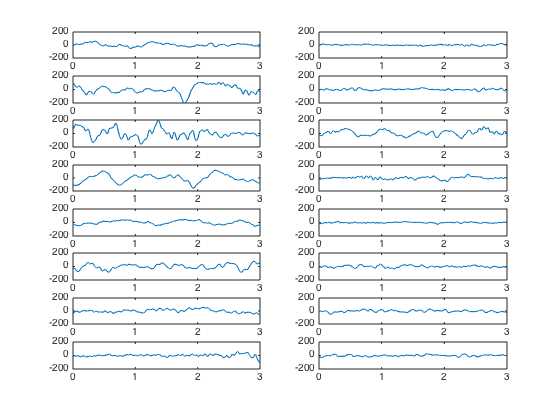
\includegraphics[width=0.6\textwidth]{figures/dataset_signals}
% \label{fig:orig}
 }
% \caption{Left: signals labeled positive ; Right: signals labeled negative.  }
\label{fig:orig}
\end{figure} 

\end{frame}

\begin{frame}{ Plan }{ Supervised learning with scattering transforms}
 \textbf{Scattering transform of the EEG signals:}  
  \begin{itemize}
   \item { Tree structured cascade of wavelet transformation operators.  The 1st order coefficients obatained from $S_1x(t,\lambda_1)=\vert x\star\psi_{\lambda}\vert \star \phi(t),$ : similar to mel-frequency spectrum. 
   }
   \item {The 2nd, 3rd,..etc levels restore information that would be otherwise lost in the first layer extraction.\\
   Example: 2nd order coefficients: $S_2x(t,\lambda_1,\lambda_2)=\vert\vert x\star \psi_{\lambda_1} \vert \star \psi_{\lambda_2}\vert \star \phi(t)$.  
   	\begin{figure}
   		\centering
   		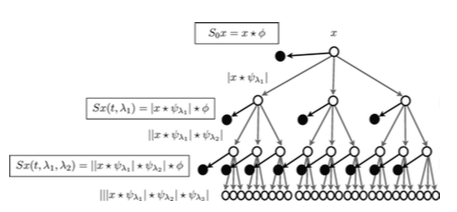
\includegraphics[scale=0.4]{figures/scat}
   		\caption{\label{fig:scat} The scatering tree visualisation.}
   	\end{figure}
   
   }
   \end{itemize}
\end{frame}


\begin{frame}{Dimensionality reduction }{ with PCA, LDA}

After Scattering transforms:
coefficients of 3 orders are aggregated to from a 46-dimensional vector. The scattering window size is chosen such that each example has $3$ aggregated feature vectors along 3 seconds.
 
 \begin{figure}[h]
    \centering
   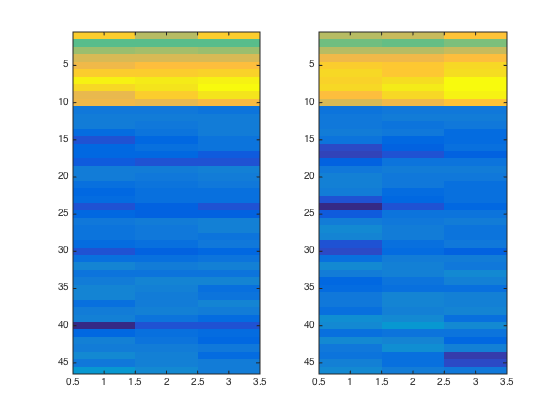
\includegraphics[scale = 0.4]{figures/dataset_coeffs}
    \label{fig:stcoeffs}
\end{figure}
\end{frame}
   
\begin{frame}{ Training and test with SVM ...}
   \begin{itemize}
   \item {  
      }
\end{itemize}
\end{frame}



\subsection{Conclusion}

%\begin{frame}{ }{Conclusion} {\small
 % \begin{itemize}
  % \item { 
   % } 
  % \item { 
%    }
   
%\end{itemize}
%} 
%\end{frame}



\section*{Summary}

% All of the following is optional and typically not needed. 
%\appendix
%\section<presentation>*{\appendixname}
%\subsection<presentation>*{For Further Reading}


\begin{frame}[allowframebreaks]{Bibliography}
\bibliographystyle{apalike}
\bibliography{beamerRef}
\end{frame}
\end{document}
